\documentclass{beamer}
\usepackage[russian]{babel}
\usetheme{metropolis}

\usepackage{hyperref}

\usepackage{amsthm}
\usepackage{ulem}
\setbeamertemplate{theorems}[numbered]

\setbeamercolor{block title}{use=structure,fg=white,bg=gray!75!black}
\setbeamercolor{block body}{use=structure,fg=black,bg=gray!20!white}

\usepackage[T2A]{fontenc}
\usepackage[utf8]{inputenc}

\usepackage{hyphenat}
\usepackage{amsmath}
\usepackage{graphicx}

\AtBeginEnvironment{proof}{\renewcommand{\qedsymbol}{}}{}{}

\title{
Микроэкономика-I
}
\author{
Павел Андреянов, PhD
}

\begin{document}

\maketitle

\begin{frame}{План лекции}
\begin{itemize}
  \item Часть 1. Экстерналии, Налоги Пигу в ЧР
  \item Часть 2. Общ. благо и уравнение Самуэльсона
\end{itemize}

\end{frame}

\section{Экстерналии}

\begin{frame}{Экстерналии}
До сих пор мы изучали экономику \alert{частного потребления}, то есть, когда потребление товара одним агентом никак не влияет на потребление (возможно, другого) товара другим агентом.

Сразу вспоминаем \alert{товары Веблена} - в них потребление товара другими агентами снижает мою полезность от частного потребления этого товара. 
\end{frame}

\begin{frame}{Экстерналии}
Попробуем описать товар Веблена:

$$U_i(x, y| \vec x_{-i}) = x + \beta y - \alpha \sum_{j \neq i} \vec x_j, \quad \alpha > 0$$
 
 
Здесь $x$ это товар Веблена, а $\tilde x_{-i}$ это вектор потребления товара $x$ другими агентами $j \neq i$.
 
Если $\alpha = 0$ то это классическая <<частная>> полезность.
\end{frame}

\begin{frame}{Экстерналии}
Попробуем описать товар Веблена:

$$U_i(x, y| \vec x_{-i}) = x + \beta y - \alpha \sum_{j \neq i} \vec x_j, \quad \alpha > 0$$
 
 
Здесь $x$ это товар Веблена, а $\tilde x_{-i}$ это вектор потребления товара $x$ другими агентами $j \neq i$. Заметим, что моя полезность падает, когда у других агентов появляется товар $x$.
 
Если $\alpha = 0$ то это классическая <<частная>> полезность.
\end{frame}

\begin{frame}{Экстерналии}
Другой пример экстерналий - \alert{эмпатийная связь}, например, между родственниками. Если $a$ и $b$ близкие родственники, с одинаковой частной полезностью $u(x,y)$ то я могу сказать, что
$$U_a(x_a, y_a | x_b, y_b) = u(x_a, y_a) + \alpha u(x_b, y_b)$$
$$U_b(x_b, y_b | x_a, y_a) = u(x_b, y_b) + \alpha u(x_a, y_a)$$
Если $\alpha = 0$ то это классическая <<частная>> полезность.
\end{frame}

\begin{frame}{Экстерналии}
Еще один пример - \alert{гонка вооружений}. Если $a$ и $b$ две воюющие страны, а $x$ это товар, представляющий собой вооружение (военные технологии), то наша полезность падает когда у противника есть вооружение
$$U_a(x_a, y_a | x_b) = u(x_a, y_a) - \alpha x_b$$
$$U_b(x_b, y_b | x_a) = u(x_b, y_b) - \alpha x_a$$
Для какой то монотонной функции $f(.)$ и $\alpha \geqslant 0$.
\end{frame}

\begin{frame}{Экстерналии}
В присутствие экстерналий, можно дать все те же определения Парето оптимальности и Равновесия Вальраса, однако, связь между ними может нарушиться.

В частности, парето фронт может как двигаться, так и стоять на месте. Равновесие Вальраса может как двигаться так и стоять на месте.
\end{frame}

\begin{frame}{Экстерналии}
В присутствие экстерналий, можно дать все те же определения Парето оптимальности и Равновесия Вальраса, однако, связь между ними может нарушиться.

Парето фронт может как двигаться, так и стоять на месте. 

РВ может как двигаться так и стоять на месте.

<<Двигаться>> с коэффициентом $\alpha$, то есть.
\end{frame}

\section{Парето Фронт}

\begin{frame}{Экстерналии}
Пусть для простоты 2 агента: $a,b$. 

Вспомним, что классический Парето фронт совпадает с решением задачи максимизации полезности
$$ U_a(x_a, y_a) + \lambda U_b(x_b,y_b) \to \max_{x_a,x_b,y_a,y_b \in E}$$
где $E$ это ящик Эджворта, а $\lambda \in [0, \infty]$. 
\end{frame}

\begin{frame}{Экстерналии}
Логика была такая: 

Если $z' = (x_a',y'_a,x'_b,y'_b)$ Парето-лучше чем $z'' = (x''_a,y''_a,x''_b,y''_b)$, то взвешенная полезность в точке $z'$ должна быть больше чем взвешенная полезность в точке $z''$, для всех строго положительных коэффициентов $\lambda$. Значит, $z''$ не может минимизировать взвешенную полезность.

Соответственно, если $z$ максимизирует взвешенную полезность, то она не может быть Парето улучшена.
\end{frame}

\begin{frame}{Экстерналии}
С экстерналиями логика не изменилась
$$ U_a(x_a, y_a|x_b, y_b) + \lambda U_b(x_b,y_b| x_a, y_a) \to \max_{x_a,x_b,y_a,y_b \in E}$$
где $E$ это ящик Эджворта, а $\lambda \in [0, \infty]$. 

В практических целях, далее и везде, \alert{будем отождествлять поиск Парето оптимума с максимизацией взвешенной полезности}, игнорируя тонкие различия между ними.
\end{frame}

\begin{frame}{Экстерналии}
Попробуем разобрать у доски два примера:
\begin{itemize}
  \item эмпатийная связь
  \item гонка вооружений
\end{itemize}
возьмем базовую полезность Кобб Дуглас.
\end{frame}

\begin{frame}{Экстерналии}

Заметим, что в случае с эмпатийной связью Парето Фронт не сдвинулся, а в случае с гонкой вооружений сдвинулся. 

Почему?

\end{frame}

\begin{frame}{Экстерналии}

На самом деле, ничего удивительного, в первом случае
\begin{gather*}
U_a(x_a, y_a|x_b, y_b) + \lambda U_b(x_b, y_b|x_a, y_a) = \\ =
u(x_a, y_a) + \alpha u(x_b, y_b) + \lambda u(x_b,y_b) + \lambda \alpha u(x_a, y_a) = \\ = (1+\lambda \alpha) u(x_a, y_a) + (\alpha + \lambda) u(x_b, y_b)\end{gather*}
То есть, это все та же максимизация взвешенной полезности, только немного изменилась параметризация кривой.

\end{frame}

\begin{frame}{Экстерналии}

Случай, когда полезность получается <<подмешиванием>> полезности другого агента с каким то коэффициентом очень специфична для моделирования родственных связей. 

В общем случае, Парето Фронт, конечно, сдвинется, просто потому что взвешенная полезность поменялась непредсказуемо.

\end{frame}


\section{Равновесие Вальраса}

\begin{frame}{Экстерналии}
Пусть для простоты 2 агента: $a,b$. 

Напомним, что в Равновесии Вальраса каждый агент максимизирует взвешенную полезность против своего бюджетного множества.
$$U_a(x_a, y_a|x_b, y_b) \to \max_{x_a, y_a}$$
$$U_b(x_b, y_b|x_a, y_a) \to \max_{x_b, y_b}$$
\end{frame}

\begin{frame}{Экстерналии}
Попробуем разобрать у доски два примера:
\begin{itemize}
  \item эмпатийная связь
  \item гонка вооружений
\end{itemize}
возьмем базовую полезность Кобб Дуглас.
\end{frame}

\begin{frame}{Экстерналии}

Получилось, что в обоих случаях Равновесие Вальраса не сдвинулось (ответ не завидел от значения коэффициента $\alpha$).

Почему?

\end{frame}

\begin{frame}{Экстерналии}
На самом деле, оба примера обладают некоторым свойством, которое можно назвать  \alert{сепарабельностью}, то есть, координаты потребления другого агента (в данном случае, аддитивно) отделены от основной полезности. 

Значения полезности прыгают по кривым безразличия агента, но сами кривые безразличия стоят на месте. 

Соответственно, решения задачи потребителя не изменилось.
\end{frame}

\begin{frame}{Экстерналии}
Попробуем придумать несепарабельный пример у доски.
\end{frame}

\section{Теорема благосостояния}

\begin{frame}{Экстерналии}
Напомню, что в случае гонки вооружений, у нас сепарабельная полезность, поэтому Равновесие Вальраса <<стоит на месте>>. 

Однако, эти полезности не являются линейной комбинацией каких-то классических полезностей, поэтому Парето Фронт <<поедет в сторону>>.

Мы только что убедились, что, в \alert{присутствие экстерналий, Равновесие Вальраса может не принадлежать Парето Фронту}.
\end{frame}

\section{Экстерналии в ЧР}

\begin{frame}{Экстерналии}
Экстерналии в частичном равновесии моделируются очень легко, \alert{как правило, это параллельный сдвиг} кривой спроса (или кривой предложения, если экстерналии на производство).

То есть, на каждую единицу товара, поверх стандартной маржинальной полезности (или маржинальных издержек) мысленно добавляются все экстерналии, положительные либо отрицательные.

Эти экстерналии зависят только от координаты <<количество Q>>, более сложные конструкции модель ЧР просто не потянет.
\end{frame}

\begin{frame}{Экстерналии}
Это учитывается при подсчете общественного благосостояния, однако, сами агенты не обращают внимания на свои экстерналии, поэтому равновесие все равно получается в старой точке пересечения (!а вовсе не в новой!). 

По моему, это никак не объясняется в курсе экономики, но мы можем сказать неформально, что экстерналии сепарабельные, поэтому агенты не меняют своего поведения.
\end{frame}

\begin{frame}{Экстерналии}
\begin{figure}[hbt]
\centering
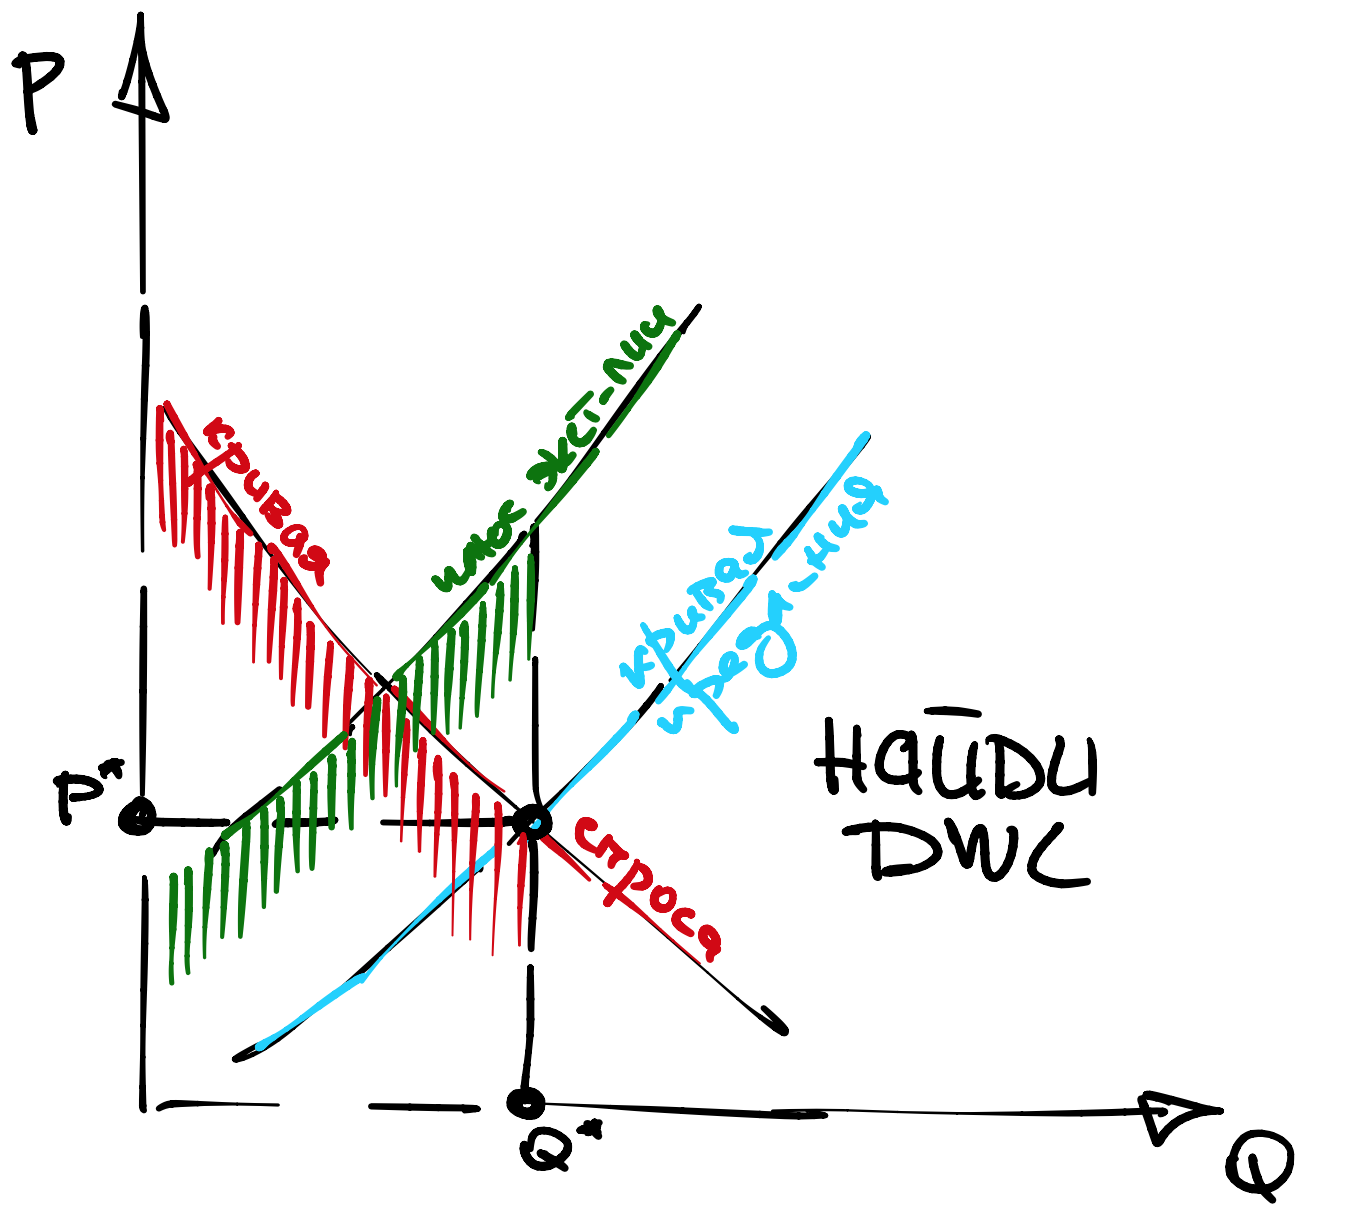
\includegraphics[width=.8 \textwidth]{dwl.png}
\end{figure}
\end{frame}

\begin{frame}{Экстерналии}
Пусть на рынке одного товара
$$ P^d(Q) = 12 - Q, \quad P^s(Q) = Q$$
Решим пару примеров:
\begin{itemize}
  \item положительные экстерналии размера 2 на единицу потребления
  \item отрицательные экстерналии размера 4 на единицу производства
\end{itemize}
Найти общественное благосостояние.
\end{frame}

\begin{frame}{Экстерналии}
Вопрос: можно ли сделать так, чтобы производство стало эффективным с учетом экстерналий?

Другими словами, чтобы $$ P = MC + \text{размер экстерналии}$$.

\end{frame}

\begin{frame}{Экстерналии}
Вопрос: можно ли сделать так, чтобы производство стало эффективным с учетом экстерналий?

Другими словами, чтобы $$ P = MC + \text{размер экстерналии.}$$
Можно!

\alert{Налог Пигу}, или корректирующий налог, это налог на любую рыночную деятельность, приводящую к отрицательным внешним эффектам (экстерналиям).

\end{frame}

\section{Налоги Пигу}

\begin{frame}{Пигу}

\begin{columns}
\begin{column}{0.5\textwidth}
   \alert{Пигу} (Arthur Cecil Pigou) английский экономист второй половины 20 века. 
   
   Работал над теорией общественного благосостояния, безработицы, бизнес циклов и много чего еще.
\end{column}
\begin{column}{0.5\textwidth}  %%<--- here
    \begin{center}
     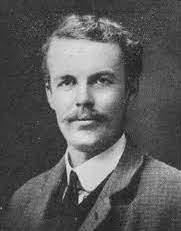
\includegraphics[width=1\textwidth]{pigou}
     \end{center}
\end{column}
\end{columns}

\end{frame}

\begin{frame}{Пигу}

Предположим, что наши экстерналии постоянны на единицу произведенного товара (как в примерах) и равны $\varepsilon$.

Что будет если ввести налог размера $\tau = \varepsilon$?

Кривая предложения переместится вверх в точности на размер экстерналий и в новом равновесии будет 
$$ P = MC + \varepsilon$$
\end{frame}

\begin{frame}{Пигу}
\begin{figure}[hbt]
\centering
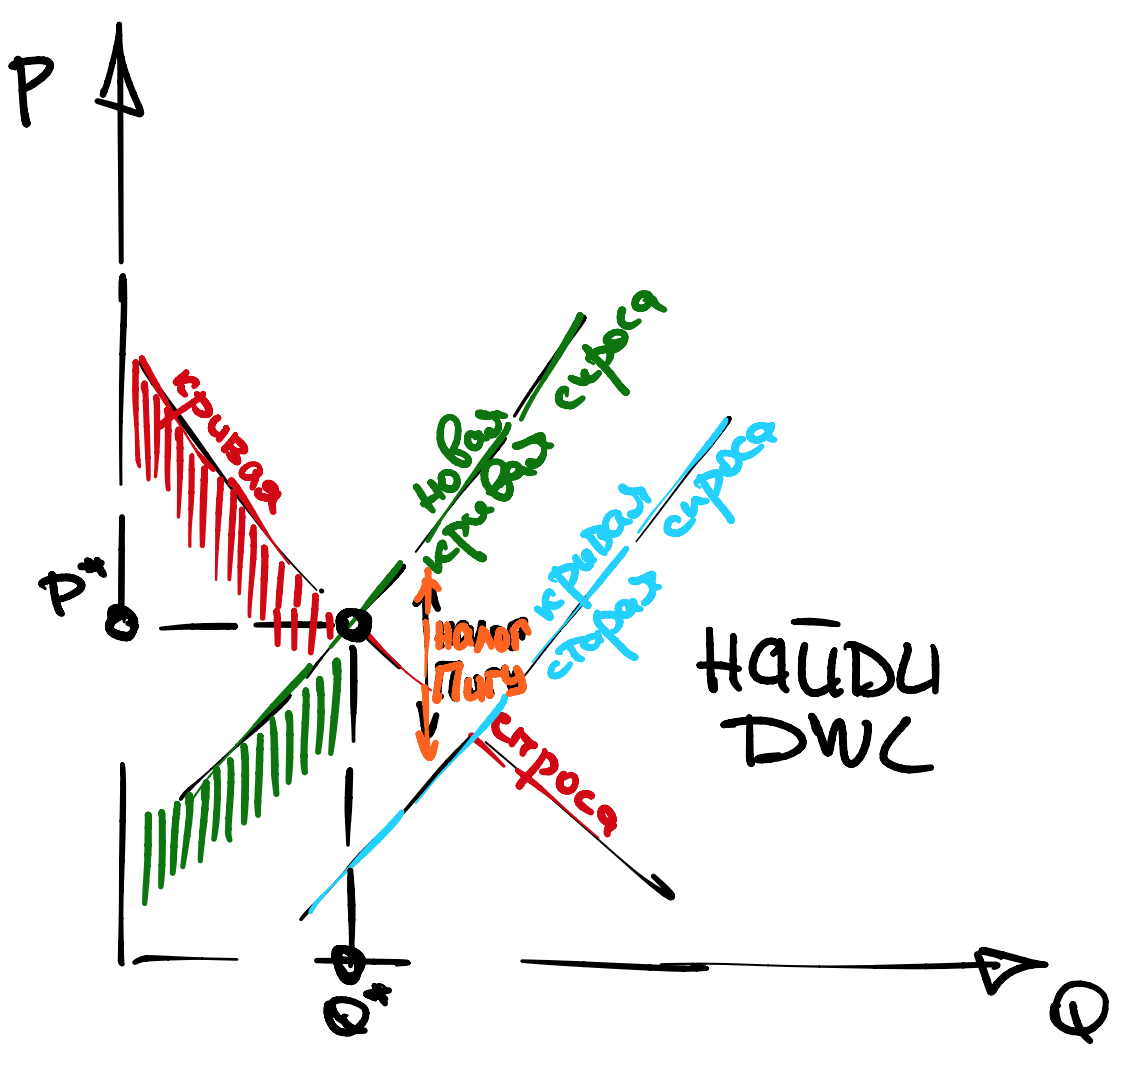
\includegraphics[width=.8 \textwidth]{dwl2.png}
\end{figure}
\end{frame}

\begin{frame}{Пигу}
Обращаю внимание, что налоги собираются положительные, а DWL исчезает. Просто замечательно!

Посчитаем благосостояние с налогами Пигу у доски.
$$ P^d(Q) = 12 - Q, \quad P^s(Q) = Q$$
и не забудем нарисовать TS на картинке
\begin{itemize}
  \item положительные экстерналии размера 2 на единицу потребления
  \item отрицательные экстерналии размера 4 на единицу производства
\end{itemize}
\end{frame}

\section{Общ. благо}

\begin{frame}{Общ. благо}
Общ. благо - это особенный вид экстерналий, когда часть полезности у всех общая. 

Классические примеры: бесплатное образование и медицина, национальная безопасность...

В контексте маленькой группы людей: интернет
\end{frame}

\begin{frame}{Общ. благо}
Рассмотрим квазилинейную полезность с общественным благом $z$
$$ U_a(x_a,y_a|z) = \log x_a + y_a + \log(z)$$
$$ U_b(x_b,y_b|z) = \log x_b + y_b + \log(z)$$
$$ y_a + y_b + y = 0, \quad x_a + x_b = 1$$
Пусть, для простоты, производством общественного блага занимается фирма с функцией издержек $y = TC(z)$. 

Мы хотим найти Парето Оптимум.
\end{frame}

\begin{frame}{Общ. благо}
Квазилинейная полезность позволяет чуть быстрее охарактеризовать ПО состояние экономики, чем это обычно делается 
\begin{gather*} \log x_a + y_a + \log(z) + \\ \lambda (\log x_b + y_b + \log(z)) + \\ \mu (-y_a - y_b - TC(z)) \to \max \end{gather*}

Из условий первого порядка: $\mu = \lambda = 1$ во внутренней точке ящика эджворта.
\end{frame}

\begin{frame}{Общ. благо}
Каждый раз, когда вы будете пытаться максимизировать взвешенную полезность при ограничении, у вас будет получаться что веса должны быть равны друг другу.

То есть,
$$ \sum_i U_i(\vec x_i, y_i, z) + (y - TC(z)) \to \max$$
не будем вдаваться в технические детали.
\end{frame}

\begin{frame}{Общ. благо}
То есть,
$$ \sum_i U_i(\vec x_i, y_i, z) + (y - TC(z)) \to \max$$
Дифференциируя по $z$ получаем
$$ \sum_i \frac{\partial}{\partial z}U_i(\vec x_i, y_i, z) = MC(z)$$
Это называется \alert{Уравнением Самуэльсона}. Если добавить к нему остальные условия первого порядка, то получится система уравнений, описывающая Парето Фронт.
\end{frame}

\begin{frame}{Общ. благо}
Но я разве только что не сказал вам, что все коэффициенты во взвешенной полезности равны друг другу?

Какой же это фронт, это больше похоже на точку!
\end{frame}

\begin{frame}{Общ. благо}
На самом деле, фронт отрисуется за счет переноса денег между агентами, а все не-денежные товары (во внутренних точках ПФ) будут константными.

Действительно, если все полезности квазилинейны (например, по вертикали) то Парето фронт это прямая (вертикальная) линия.

Так у вас было в одной из домашек.
\end{frame}

\section{Общ. благо в ЧР}

\begin{frame}{Общ. благо}
В модели частичного равновесия, когда речь идет об эффективном производстве \alert{частного блага}, мы обычно пересекаем суммарный спрос с кривой предложения.

Причем, \alert{суммирование по горизонтали}.

Получается привычная нам картинка.
\end{frame}

\begin{frame}{Общ. благо}
\begin{figure}[hbt]
\centering
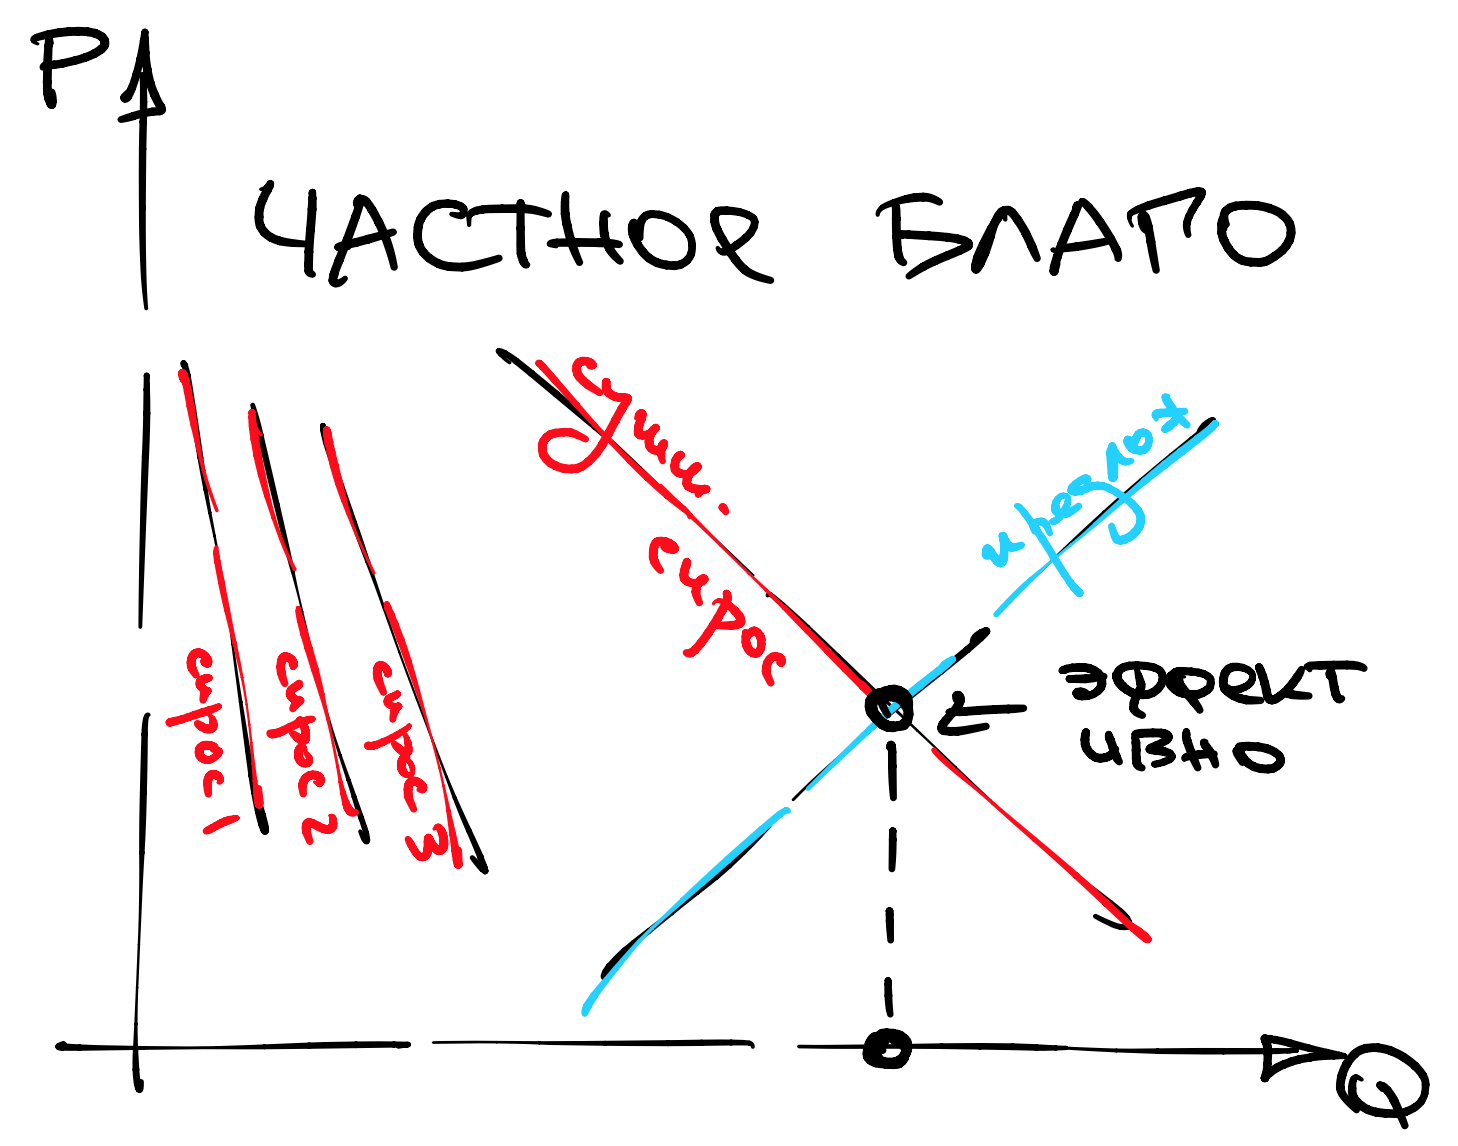
\includegraphics[width=.9 \textwidth]{private.png}
\end{figure}
\end{frame}

\begin{frame}{Общ. благо}
В модели частичного равновесия, когда речь идет об эффективном производстве \alert{общественного товара}, мы также пересекаем суммарный спрос с кривой предложения.

Однако, в этот раз \alert{суммирование по вертикали}.

Это, на самом деле, и есть уравнение Самуэльсона, оно говорит что сумма предельных полезностей от потребления общественного блага равно маржинальным издержкам по его производству.
\end{frame}

\begin{frame}{Общ. благо}
\begin{figure}[hbt]
\centering
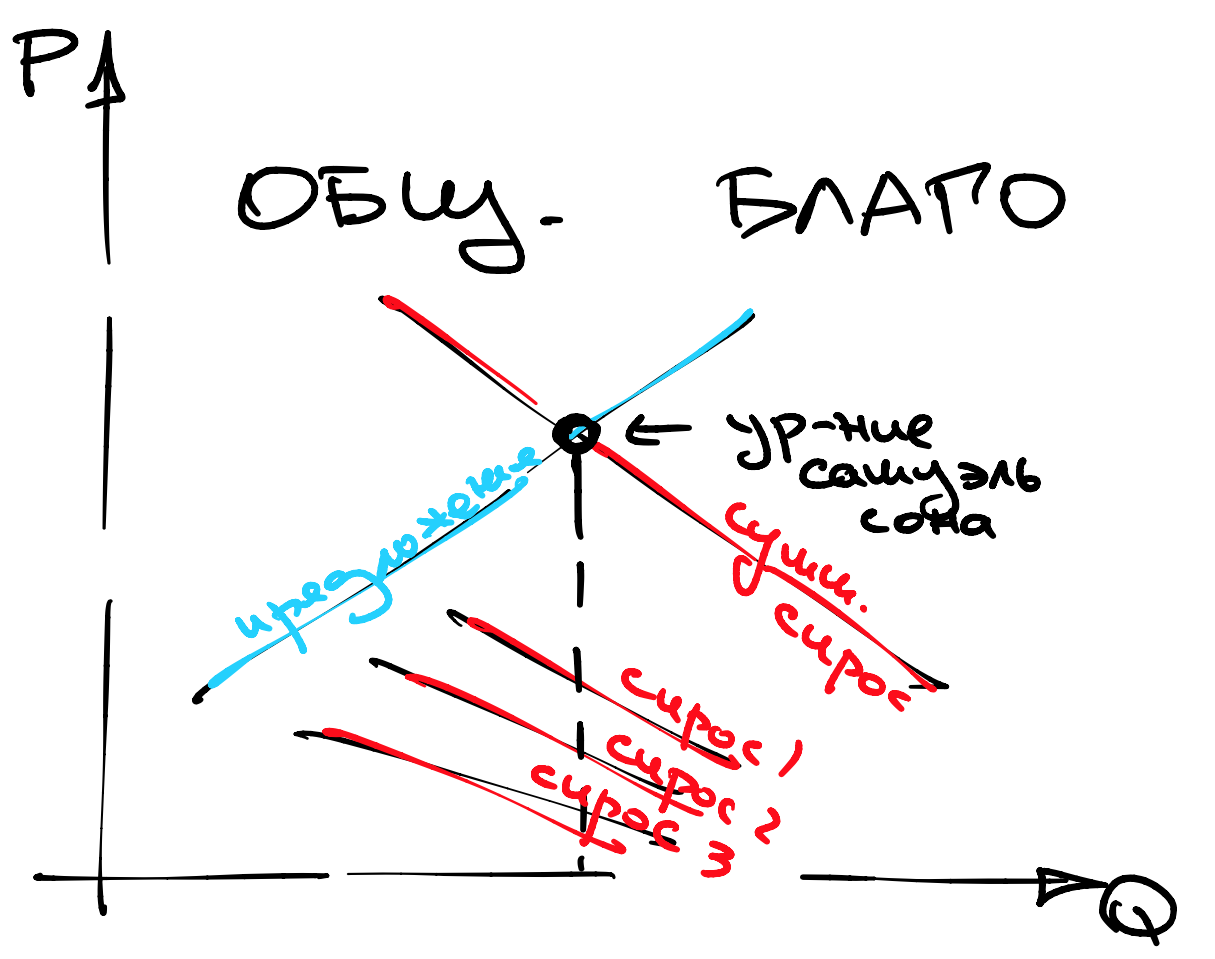
\includegraphics[width=.9 \textwidth]{public.png}
\end{figure}
\end{frame}

\begin{frame}{Общ. благо}
Потренируемся посчитать CS, PS:

\begin{itemize}
  \item предложение: $P = Q$
  \item (обратный) спрос первого агента: $P = 10 - Q$ 
  \item (обратный) спрос второго агента: $P = 10 - 2Q$ 
\end{itemize}
\end{frame}

\begin{frame}{Общ. благо}
Остается вопрос оплаты общественного блага. Это очень нетривиальная задача, и есть много разных попыток ее разрешить:
\begin{itemize}
  \item разделить стоимость поровну
  \item разделить стоимость пропорционально полезностям
  \item разделить стоимость пропорционально вектору шэпли
\end{itemize}
но неочевидно, что все на это согласятся, или что что все захотят сообщить свои истинные полезности.
\end{frame}

\section{Общ. благо в ОР}

\begin{frame}{Общ. благо}
В более общем случае, выберем один товар $x_0$, он не обязан быть квазилинейным. 

Пусть, для простоты, единственное общественное благо $z$ и производится согласно технологии
$$ F(\vec X, z) \leqslant 0, \quad X = (X_0,X_1, \ldots, X_n)$$
Мы хотим просто выписать уравнение Самуэльсона.
\end{frame}

\begin{frame}{Общ. благо}
Тогда классические условия первого порядка говорят что, для любого агента $i$ и любого товара $k \neq 0$:
$$ \frac{\partial}{\partial x_k} U_i(\vec x, z)/\frac{\partial}{\partial x_0} U_i(\vec x, z) = \frac{\partial}{\partial X_k} F(\vec X, z)/\frac{\partial}{\partial X_0} F(\vec X, z)$$
А \alert{уравнение Самуэльсона} (выведем у доски методом МЛ)
$$ \sum_{i \in I} \frac{\partial}{\partial z} U_i(\vec x, z)/\frac{\partial}{\partial x_0} U_i(\vec x, z) = \frac{\partial}{\partial z} F(\vec X, z)/\frac{\partial}{\partial X_0} F(\vec X, z)$$
в квазилинейном случае знаменатели просто были равны нулю.
\end{frame}

\begin{frame}{Общ. благо}
Напоследок, расскажу о попытке сформулировать аналог Равновесия Вальраса с общественным благом. Это называется \alert{равновесием Линдаля}.

Для этого, для каждого общественного блага $z$ нам понадобится не только новая цена $q$ а еще (вдобавок) целый вектор $\vec q = \{q_i\}_{i \in I}$.
\end{frame}

\begin{frame}{Общ. благо}
Соответственном если у вас, например, $K$ частных благ, $I$ агентов и одно общественное благо, то вам понадобится $K+I-1$ цен (единичка вычитается из за нормировки).

Каждый агент видит свою индивидуальную цену общественного блага $q_i$ а фирма (или фирмы) видят одну единственную цену $q$.
\end{frame}

\begin{frame}{Общ. благо}
\alert{Равновесие Линдаля} это такой набор цен частных и общественных благ, что 

\begin{itemize}
  \item выполнены товарные равенства
  \item каждый агент максимизирует полезность, не обращая внимание на природу общественного блага
  \item фирма максимизирует прибыль
  \item каждый агент (добровольно) покупает одно и то же количество общественного блага
  \item $\sum_{i=I} q_i = q$
\end{itemize}

\end{frame}

\begin{frame}{Общ. благо}
Обратим внимание на последнее уравнение:
$$\sum_{i=I} q_i = q$$
Это, на самом деле, уравнение Самуэльсона (проще увидеть в квазилинейном случае $\sum_{i = I} MU_i = MC$) и оно гарантирует, что мы окажемся на Парето Фронте.

\end{frame}

%\section{Налоги Пигу в ОР}
%
%\begin{frame}{Пигу}
%
%В общем равновесии ситуация немного более сложная.
%
%Вообще непонятно,
%
%\begin{itemize}
%  \item какую цель преследуем?
%  \item на сколько товаров ввести налог?
%  \item налоги индивидуальные или общие?
%\end{itemize}
%
%\end{frame}
%
%\begin{frame}{Пигу}
%Короткий ответ:
%\begin{itemize}
%  \item какую цель преследуем? попасть на ПФ
%  \item на сколько товаров ввести налог???
%  \item налоги индивидуальные или общие? индивидуальные
%\end{itemize}
%При этом, хотелось бы собрать в точности 0 налогов, чтобы сохранить денежное равенство.
%\end{frame}
%
%\begin{frame}{Пигу}
%Рассмотрим положительные экстерналии на потребление в экономике обмена:
%$$U_a(x_a,y_a|x_b)= \log x_a + \log y_a + \log x_b, \quad U_b(x_b,y_b) = \log x_b + \log y_b$$
%общие запасы пусть равняются $(1,1)$. \end{frame}
%
%\begin{frame}{Пигу}
%Найдем Парето Фронт
%$$ U_a(x_a,y_a|1-x_a) + \lambda U_b(1-x_a,1-y_a) \to \max$$
%Запишем условия первого порядка
%$$ \log x_a + \log y_a + \log (1-x_a) + \lambda (\log (1-x_a) + \log (1-y_a)) \to \max$$
%$$ \frac{1}{x_a} = \frac{\lambda + 1}{1-x_a}, \quad \frac{1}{y_a} = \frac{\lambda}{1-y_a}
%$$
%что приведет к
%$$ x_a = \frac{1}{2+\lambda}, \quad y_a = \frac{1}{1+\lambda},$$
%$$ x_b = 1-\frac{1}{2+\lambda}, \quad y_b = 1-\frac{1}{1+\lambda},$$
%мы хотели бы туда попасть.
%\end{frame}
%
%\begin{frame}{Пигу}
%Теперь найдем РВ (пусть нач. запасы равны (1,0), (0,1)).
%
%Пусть налоги индивидуальны, скажем, $\tau$ это налог на товар $x$ агенту $a$, а цены равны $(p,1)$. 
%
%Уточним, что запасы продаются по тем же ценам, что и покупаются, поэтому денежное равенство будет выполнено.
%\end{frame}
%
%\begin{frame}{Пигу}
%\begin{gather*}x_a = \frac{1}{p+\tau}\frac{p+\tau+1}{2} = \frac{1}{2+\lambda},\\ y_a = \frac{1}{1}\frac{p+\tau+1}{2} = \frac{1}{1+\lambda} \\
%x_b = \frac{1}{p}\frac{p+1}{2} = 1-\frac{1}{2+\lambda},\\ y_b = \frac{1}{1}\frac{p+1}{2} = 1-\frac{1}{1+\lambda}
%\end{gather*}
%Уравнения 3,4 уравнение дают нам $\lambda, p$. 
%
%А 1 или 2 дают нам $\tau = 6$.
%\end{frame}

\end{document}
